% Created by tikzDevice version 0.12.6 on 2025-04-07 11:17:38
% !TEX encoding = UTF-8 Unicode
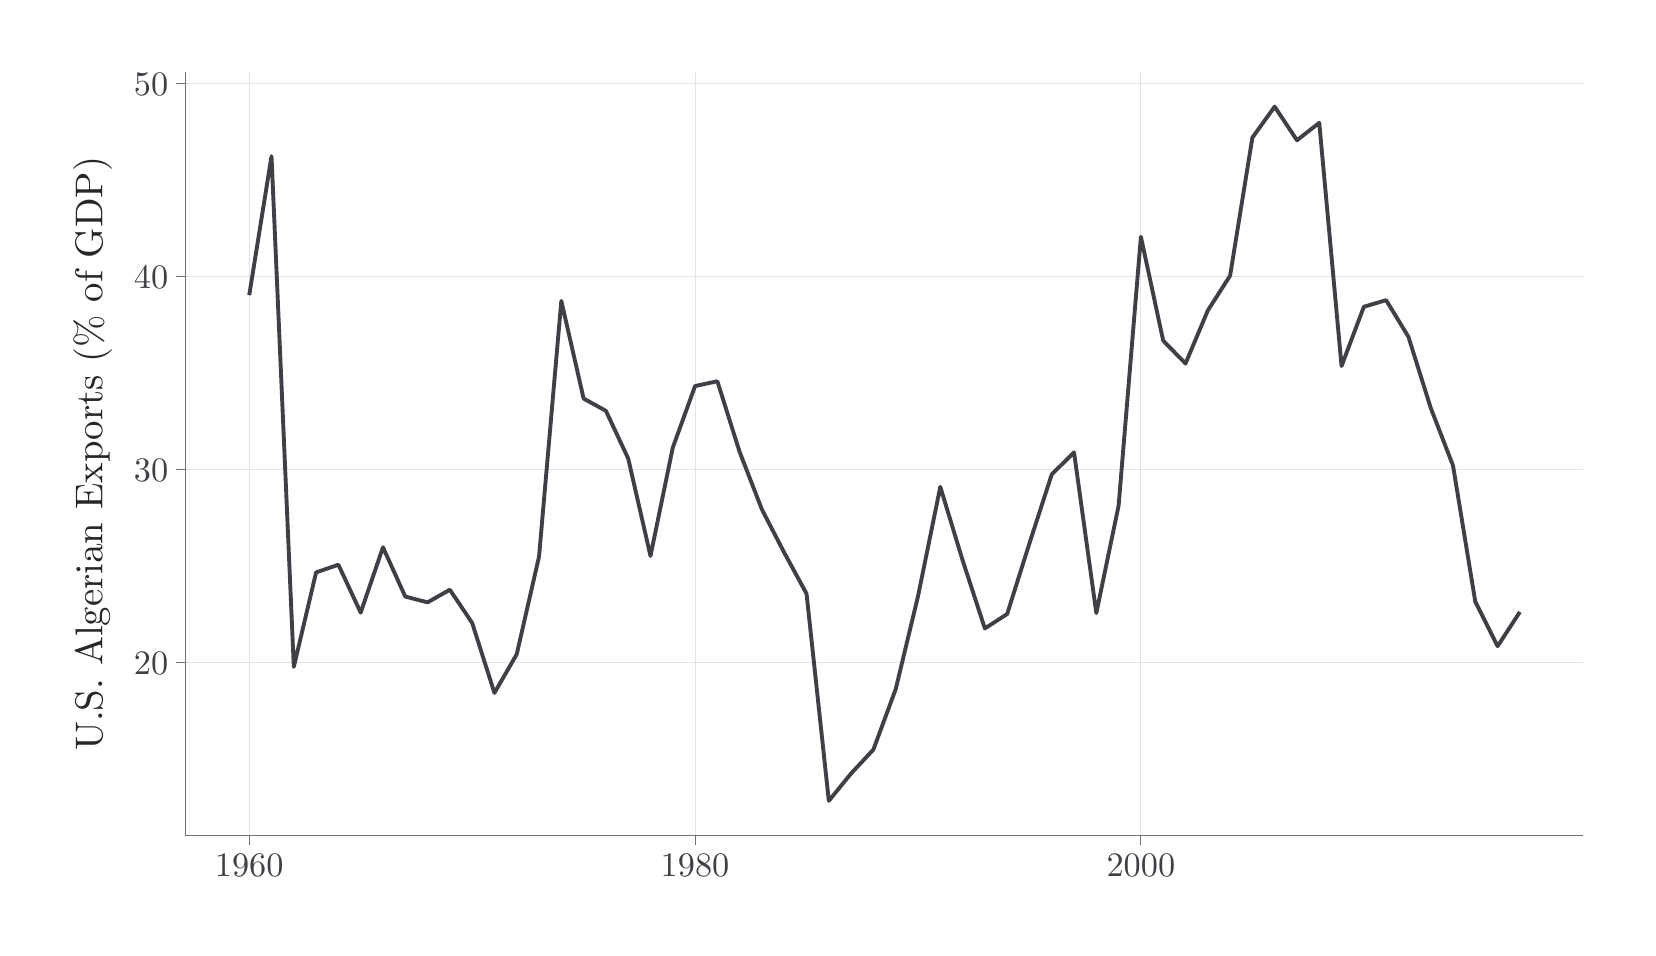
\begin{tikzpicture}[x=1pt,y=1pt]
\definecolor{fillColor}{RGB}{255,255,255}
\path[use as bounding box,fill=fillColor] (0,0) rectangle (578.16,325.21);
\begin{scope}
\path[clip] (  0.00,  0.00) rectangle (578.16,325.21);
\definecolor{drawColor}{RGB}{255,255,255}

\path[draw=drawColor,line width= 0.7pt,line join=round,line cap=round,fill=fillColor] (  0.00,  0.00) rectangle (578.16,325.21);
\end{scope}
\begin{scope}
\path[clip] ( 57.10, 33.29) rectangle (562.16,309.21);
\definecolor{drawColor}{RGB}{255,255,255}
\definecolor{fillColor}{RGB}{255,255,255}

\path[draw=drawColor,line width= 0.7pt,line join=round,line cap=round,fill=fillColor] ( 57.10, 33.29) rectangle (562.16,309.22);
\definecolor{drawColor}{RGB}{228,228,231}

\path[draw=drawColor,line width= 0.4pt,line join=round] ( 57.10, 95.68) --
	(562.16, 95.68);

\path[draw=drawColor,line width= 0.4pt,line join=round] ( 57.10,165.44) --
	(562.16,165.44);

\path[draw=drawColor,line width= 0.4pt,line join=round] ( 57.10,235.21) --
	(562.16,235.21);

\path[draw=drawColor,line width= 0.4pt,line join=round] ( 57.10,304.97) --
	(562.16,304.97);

\path[draw=drawColor,line width= 0.4pt,line join=round] ( 80.06, 33.29) --
	( 80.06,309.21);

\path[draw=drawColor,line width= 0.4pt,line join=round] (241.16, 33.29) --
	(241.16,309.21);

\path[draw=drawColor,line width= 0.4pt,line join=round] (402.26, 33.29) --
	(402.26,309.21);
\definecolor{drawColor}{RGB}{63,63,70}

\path[draw=drawColor,line width= 1.4pt,line join=round] ( 80.06,228.53) --
	( 88.11,278.77) --
	( 96.17, 94.24) --
	(104.22,128.36) --
	(112.28,131.15) --
	(120.33,113.84) --
	(128.39,137.44) --
	(136.44,119.64) --
	(144.50,117.55) --
	(152.55,122.11) --
	(160.61,110.14) --
	(168.66, 84.81) --
	(176.72, 98.81) --
	(184.78,134.07) --
	(192.83,226.48) --
	(200.89,191.18) --
	(208.94,186.75) --
	(217.00,169.53) --
	(225.05,134.30) --
	(233.11,173.45) --
	(241.16,195.71) --
	(249.22,197.44) --
	(257.27,171.89) --
	(265.33,151.08) --
	(273.38,135.51) --
	(281.44,120.68) --
	(289.49, 45.83) --
	(297.55, 55.72) --
	(305.60, 64.34) --
	(313.66, 86.18) --
	(321.71,119.70) --
	(329.77,159.29) --
	(337.82,132.79) --
	(345.88,108.12) --
	(353.93,113.33) --
	(361.99,138.89) --
	(370.04,163.77) --
	(378.10,171.76) --
	(386.15,113.66) --
	(394.21,152.54) --
	(402.26,249.64) --
	(410.32,212.11) --
	(418.38,203.84) --
	(426.43,222.99) --
	(434.49,235.58) --
	(442.54,285.47) --
	(450.60,296.67) --
	(458.65,284.52) --
	(466.71,290.83) --
	(474.76,202.92) --
	(482.82,224.35) --
	(490.87,226.74) --
	(498.93,213.51) --
	(506.98,187.83) --
	(515.04,166.97) --
	(523.09,117.80) --
	(531.15,101.68) --
	(539.20,114.09);
\end{scope}
\begin{scope}
\path[clip] (  0.00,  0.00) rectangle (578.16,325.21);
\definecolor{drawColor}{RGB}{113,113,122}

\path[draw=drawColor,line width= 0.3pt,line join=round] ( 57.10, 33.29) --
	( 57.10,309.21);
\end{scope}
\begin{scope}
\path[clip] (  0.00,  0.00) rectangle (578.16,325.21);
\definecolor{drawColor}{RGB}{63,63,70}

\node[text=drawColor,anchor=base east,inner sep=0pt, outer sep=0pt, scale=  1.24] at ( 50.80, 91.39) {20};

\node[text=drawColor,anchor=base east,inner sep=0pt, outer sep=0pt, scale=  1.24] at ( 50.80,161.16) {30};

\node[text=drawColor,anchor=base east,inner sep=0pt, outer sep=0pt, scale=  1.24] at ( 50.80,230.92) {40};

\node[text=drawColor,anchor=base east,inner sep=0pt, outer sep=0pt, scale=  1.24] at ( 50.80,300.69) {50};
\end{scope}
\begin{scope}
\path[clip] (  0.00,  0.00) rectangle (578.16,325.21);
\definecolor{drawColor}{RGB}{113,113,122}

\path[draw=drawColor,line width= 0.3pt,line join=round] ( 53.60, 95.68) --
	( 57.10, 95.68);

\path[draw=drawColor,line width= 0.3pt,line join=round] ( 53.60,165.44) --
	( 57.10,165.44);

\path[draw=drawColor,line width= 0.3pt,line join=round] ( 53.60,235.21) --
	( 57.10,235.21);

\path[draw=drawColor,line width= 0.3pt,line join=round] ( 53.60,304.97) --
	( 57.10,304.97);
\end{scope}
\begin{scope}
\path[clip] (  0.00,  0.00) rectangle (578.16,325.21);
\definecolor{drawColor}{RGB}{113,113,122}

\path[draw=drawColor,line width= 0.3pt,line join=round] ( 57.10, 33.29) --
	(562.16, 33.29);
\end{scope}
\begin{scope}
\path[clip] (  0.00,  0.00) rectangle (578.16,325.21);
\definecolor{drawColor}{RGB}{113,113,122}

\path[draw=drawColor,line width= 0.3pt,line join=round] ( 80.06, 29.79) --
	( 80.06, 33.29);

\path[draw=drawColor,line width= 0.3pt,line join=round] (241.16, 29.79) --
	(241.16, 33.29);

\path[draw=drawColor,line width= 0.3pt,line join=round] (402.26, 29.79) --
	(402.26, 33.29);
\end{scope}
\begin{scope}
\path[clip] (  0.00,  0.00) rectangle (578.16,325.21);
\definecolor{drawColor}{RGB}{63,63,70}

\node[text=drawColor,anchor=base,inner sep=0pt, outer sep=0pt, scale=  1.24] at ( 80.06, 18.42) {1960};

\node[text=drawColor,anchor=base,inner sep=0pt, outer sep=0pt, scale=  1.24] at (241.16, 18.42) {1980};

\node[text=drawColor,anchor=base,inner sep=0pt, outer sep=0pt, scale=  1.24] at (402.26, 18.42) {2000};
\end{scope}
\begin{scope}
\path[clip] (  0.00,  0.00) rectangle (578.16,325.21);
\definecolor{drawColor}{RGB}{39,39,42}

\node[text=drawColor,rotate= 90.00,anchor=base,inner sep=0pt, outer sep=0pt, scale=  1.40] at ( 27.00,171.25) {U.S. Algerian Exports (\% of GDP)};
\end{scope}
\end{tikzpicture}
